Основной этап поиска кандидатов -- это отбор звёзд, соответствующих нижеизложенным критериям. Для этого необходимо наличие информации лишь о звёздной величине кандидатов в ультрафиолетовом и инфракрасном спектральных диапазонах, а спектральные данные не требуются.

При создании критериев мы будем придерживаться следующей модели. Взяв за образец выборку известных звёзд типа Т Тельца, находящихся на небольшом расстоянии, мы определим положение этих звёзд на цветовых диаграммах. Все источники, попавшие в ту же область диаграммы цвет-цвет, мы сочтём первичными кандидатами, определив условные границы этой области.

В основе данной модели составления критериев лежит работа Гомез де Кастро 2014 [ссылка], в которой аналогичное исследование проводится для молекулярного облака Тельца.

\section{Эталонная выборка}
Чтобы определить, какого поведения мы ожидаем от кандидатов в T Tauri звёзды, нам понадобится образцовая выборка, состоящая из известных и подтверждённых T Tauri звёзд.

Мы возьмём звёзды, наблюдавшиеся телескопом IUE (International Ultraviolet Explorer). Выборка из 21 звезды получена в работе [Gomez de Castro $\&$ Franqueira 1997]. Далее их IUE спектры были умножены на функцию пропускания фильтров GALEX [Ana Ines]. 

...формулы эти может...

\begin{table}[ht]
\caption{Эталонная выборка звёзд, используемых как образец для формулирования критериев.}
\label{tabular:etalon}
\begin{center}
\begin{tabular}{cccccccccc}
Star & Spectral & d & FUV & NUV & R & J & H & K \\
 &  type & pc & AB mag & AB  mag & mag & mag & mag & mag \\
WY Ari & K5 Bin & 275 & 17.36 & 15.26 & 12.40 & 10.229 & 9.418 & 8.901 \\
BP Tau & K7 & 140 & 17.66 & 15.97 & 11.62 & 9.10 & 8.22 & 7.736 \\
DE Tau & M2 & 140 & 17.96 & 16.49 & 11.93 & 9.18 & 8.273 & 7.799 \\
RY Tau & K1 & 140 & 17.73 & 15.38 & 9.67 & 7.16 & 6.13 & 5.395 \\
T Tau & K0 & 140 & 16.42 & 14.97 & 9.80 & 7.24 & 6.237 & 5.325 \\
DF Tau & M0-1 & 140 & 17.58 & 16.78 & 11.50 & 8.17 & 7.256 & 6.734 \\
DR Tau & K4 & 140 & 16.95 & 14.87 & 12.19 & 8.85 & 7.8 & 6.874 \\
GM Aur & K3 & 140 & 17.57 & 16.39 & 11.22 & 9.34 & 8.603 & 8.283 \\
SU Aur & G2 & 140 & 18.04 & 15.21 & 9.17 & 7.20 & 6.558 & 5.99 \\
RW Aur & K1 & 140 & 16.51 & 14.13 & 9.95 & 8.38 & 7.621 & 7.02 \\
GW Ori & G5 & 450 & 17.44 & 15.02 & 9.52 & 7.70 & 7.103 & 6.59 \\
CV Cha & G8 & 175 & 17.32 & 14.94 & 10.51 & 8.29 & 7.46 & 6.845 \\
RU Lup & K7 & 140 & 15.85 & 13.41 & 9.99 & 8.73 & 7.824 & 7.138 \\
AK Sco & F5 SB & 145 & 17.15 & 14.01 & 9.20 & 7.68 & 7.06 & 6.503 \\
DI Cep & G8 & 244 & 17.51 & 15.11 & 10.49 & 9.30 & 8.572 & 7.952 \\
HD 283572 & G5 & 140 & 18.75 & 14.77 & 9.14 & 7.41 & 7.008 & 6.869 \\
AB Dor & K0 & 15 & 16.32 & 12.8 & 6.50 & 5.32 & 4.845 & 4.686 \\
TW Hya & K7 & 56 & 15.65 & 14 & 10.19 & 8.22 & 7.558 & 7.297 \\
V2398 Oph & G8 & 125 & 16.23 & 14.48 & 10.10 & 8.62 & 7.81 & 7.23 \\
V4046 Sgr & K5.6 SB & 83 & 16.6 & 16.05 & 9.67 & 8.07 & 7.435 & 7.249 \\
FK Ser & K7 Bin & 350 & 17.72 & 16.19 & 9.41 & 7.64 & 6.92 & 6.624 \\
\end{tabular}
\end{center}
\end{table}

В эталонной выборке содержится мало WTTS и звёзд M типа, что обусловлено низкой чувствительностью телескопа IUE. Можно заметить, что в FUV звёздная величина мала, это делает более трудным поиск звёзд типа Т Тельца со слабыми линиями.

\section{Цветовые диаграммы и критерии отбора}
Перейдём к построению диаграмм цвет-цвет. Мы используем четыре типа этих диаграмм: FUV-NUV vs J-K, FUV-NUV vs H-K, NUV-H vs J-K и NUV-R vs J-K. Первые три существенны для отделения кандидатов, четвёртый же выполняет иллюстративную функцию, так как на диаграмму этого типа, требующую наличия блеска в фильтре R, попадает гораздо меньше звёзд.

\begin{figure}[ht]
\begin{minipage}[ht]{0.49\linewidth}
\center{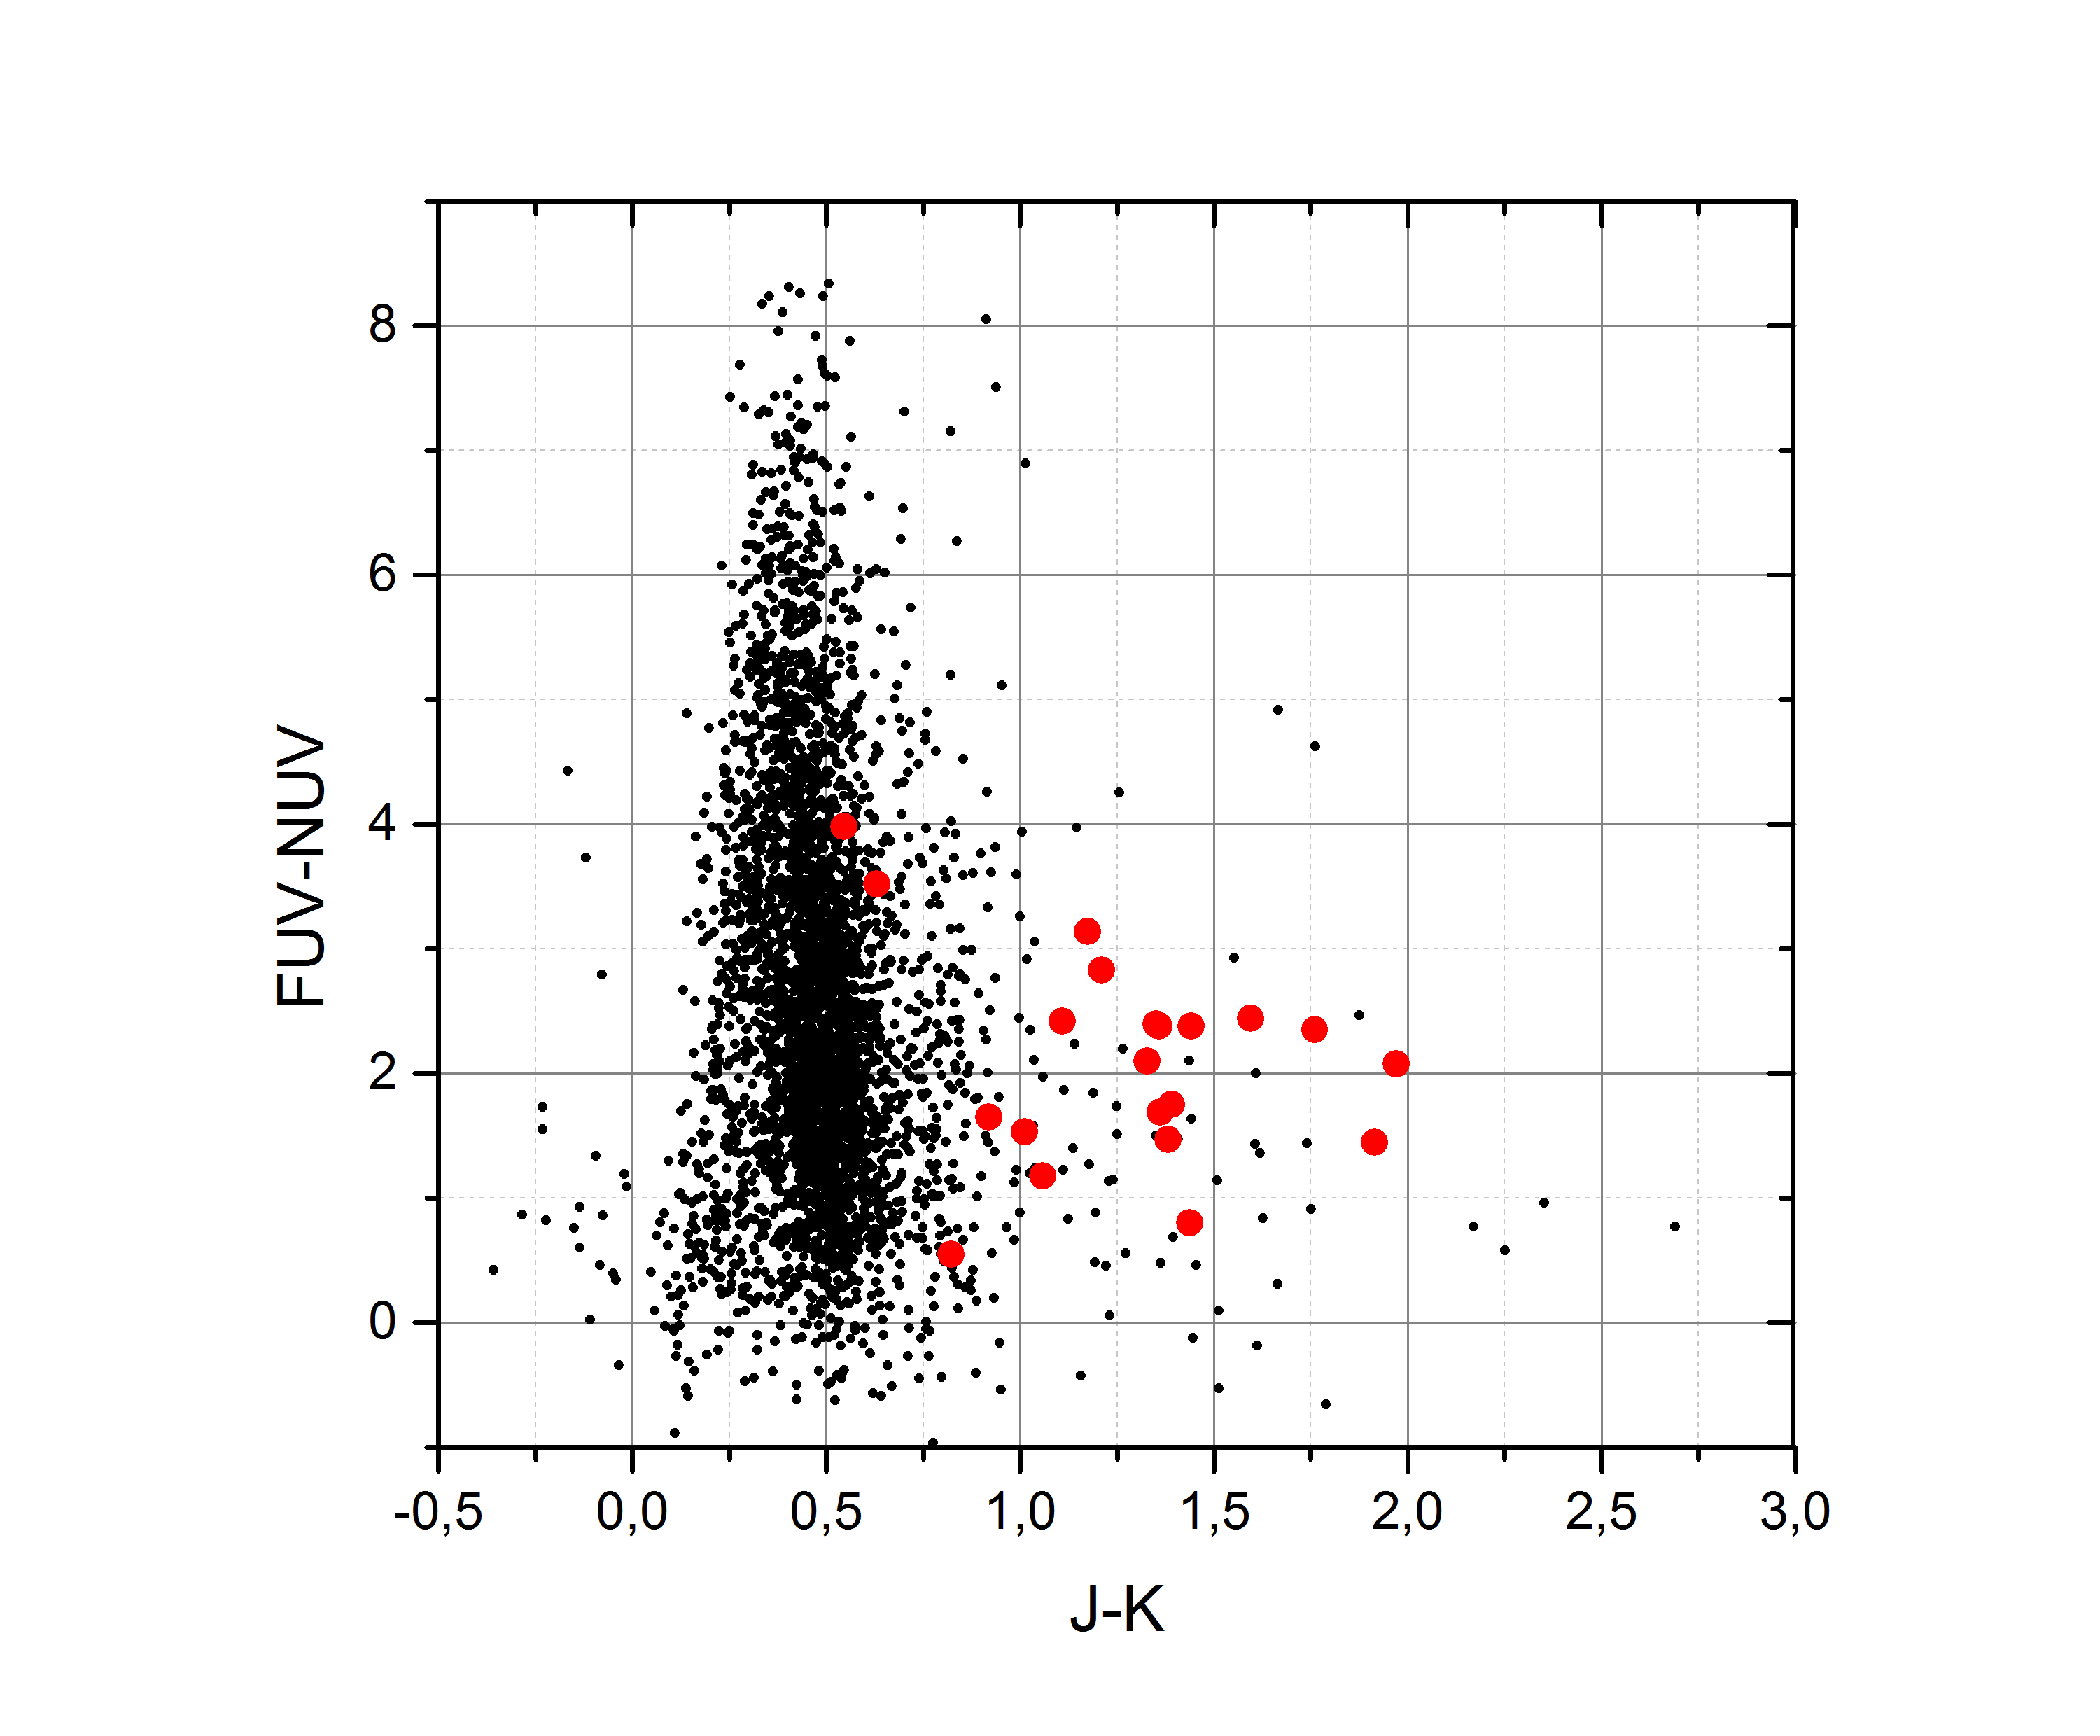
\includegraphics[width=1\linewidth]{Graph1.png} \\ FUV-NUV vs J-K}
\end{minipage}
\hfill
\begin{minipage}[ht]{0.49\linewidth}
\center{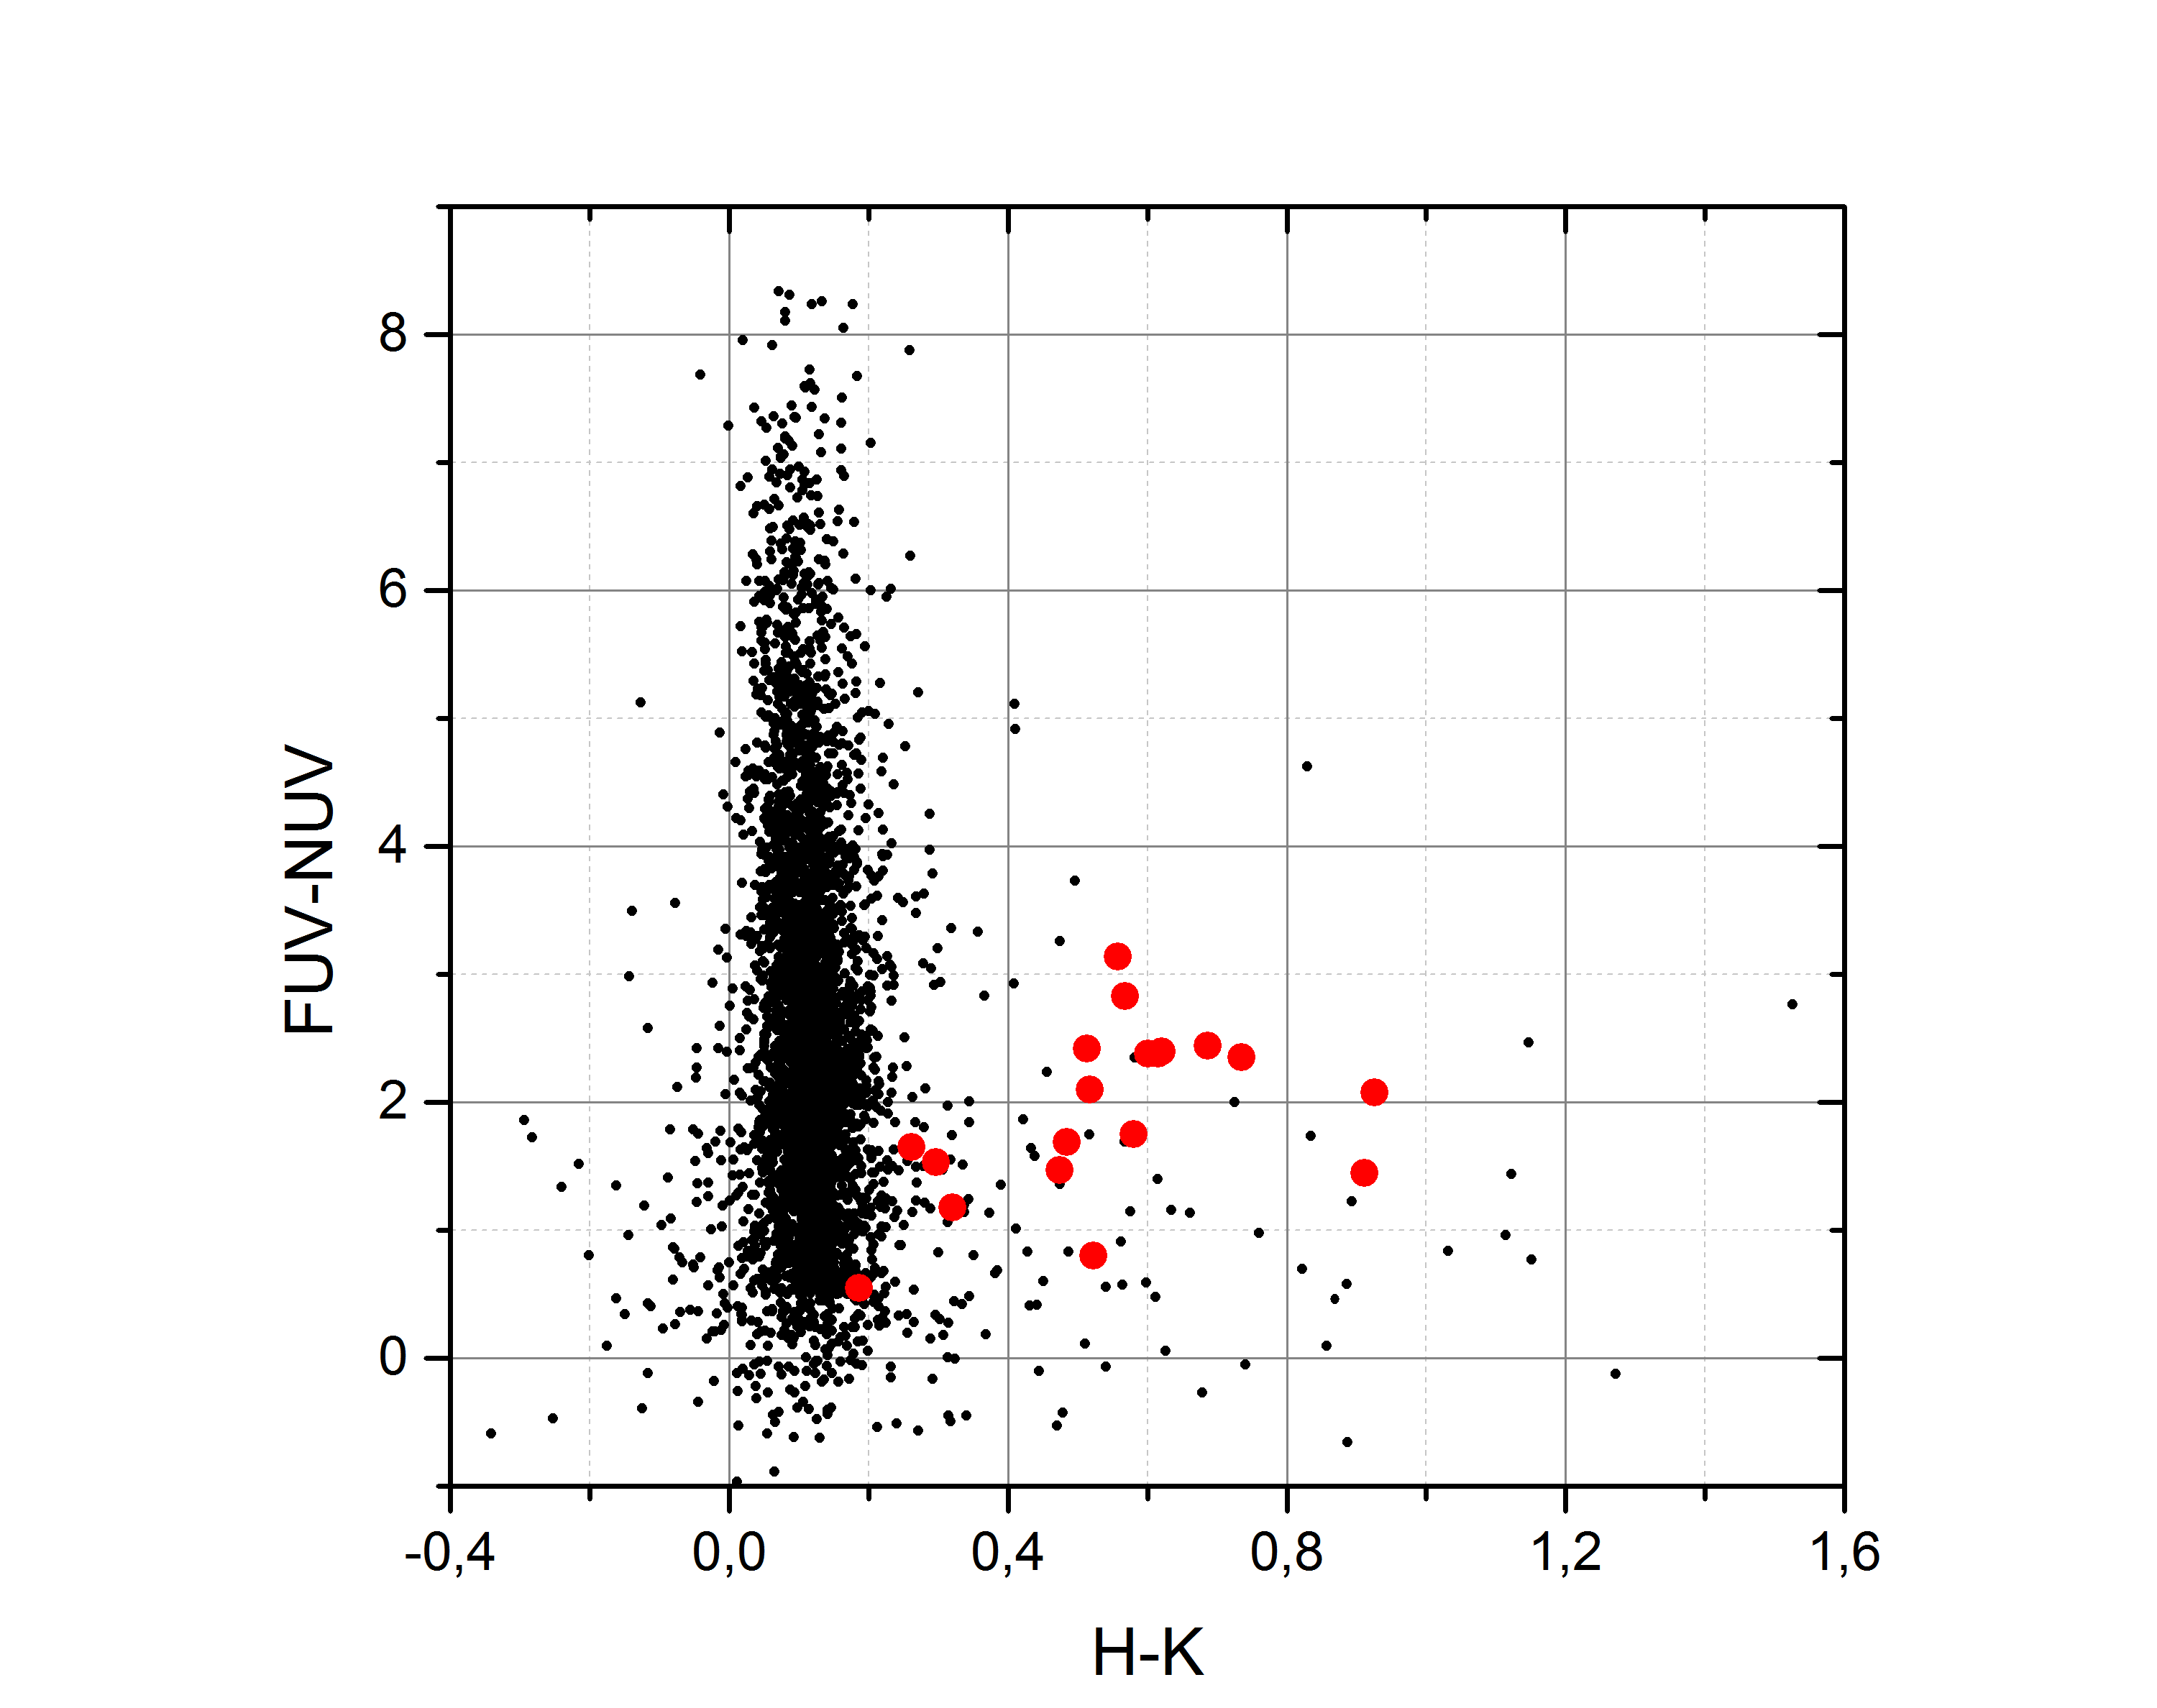
\includegraphics[width=1\linewidth]{Graph2.png} \\ FUV-NUV vs H-K}
\end{minipage}
\begin{minipage}[ht]{0.49\linewidth}
\center{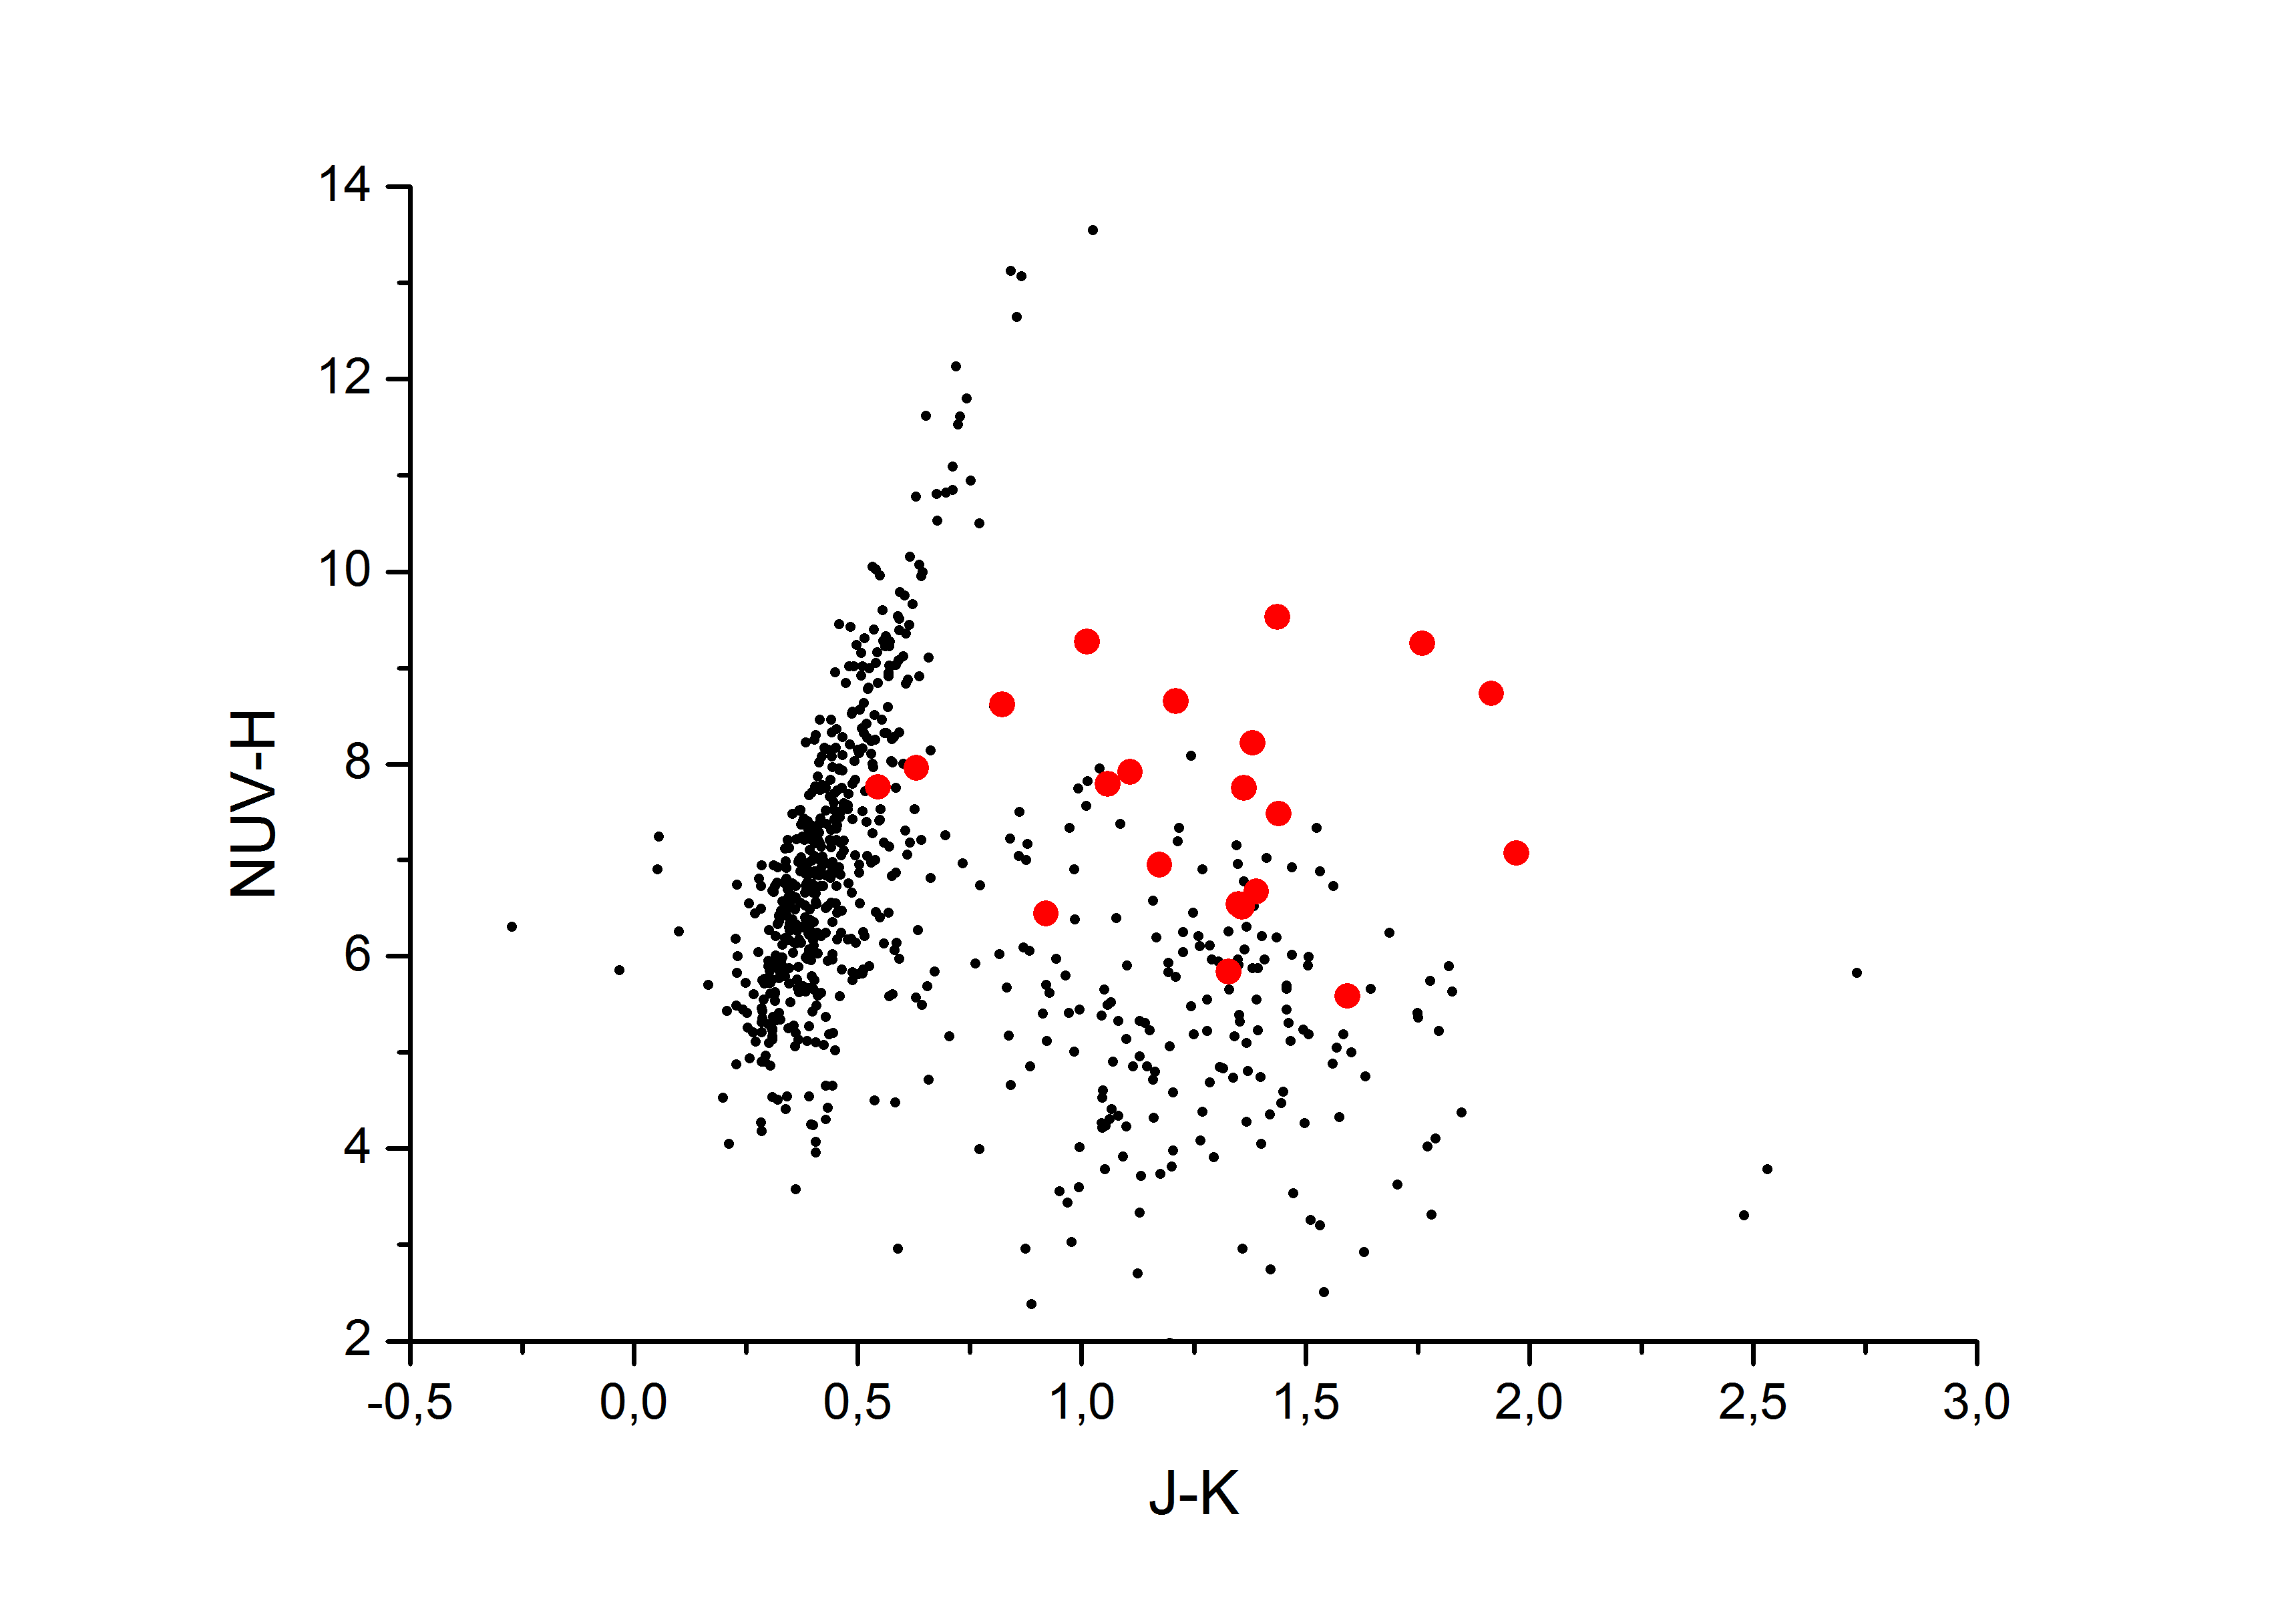
\includegraphics[width=1\linewidth]{Graph3.png} \\ NUV-H vs J-K}
\end{minipage}
\hfill
\begin{minipage}[ht]{0.49\linewidth}
\center{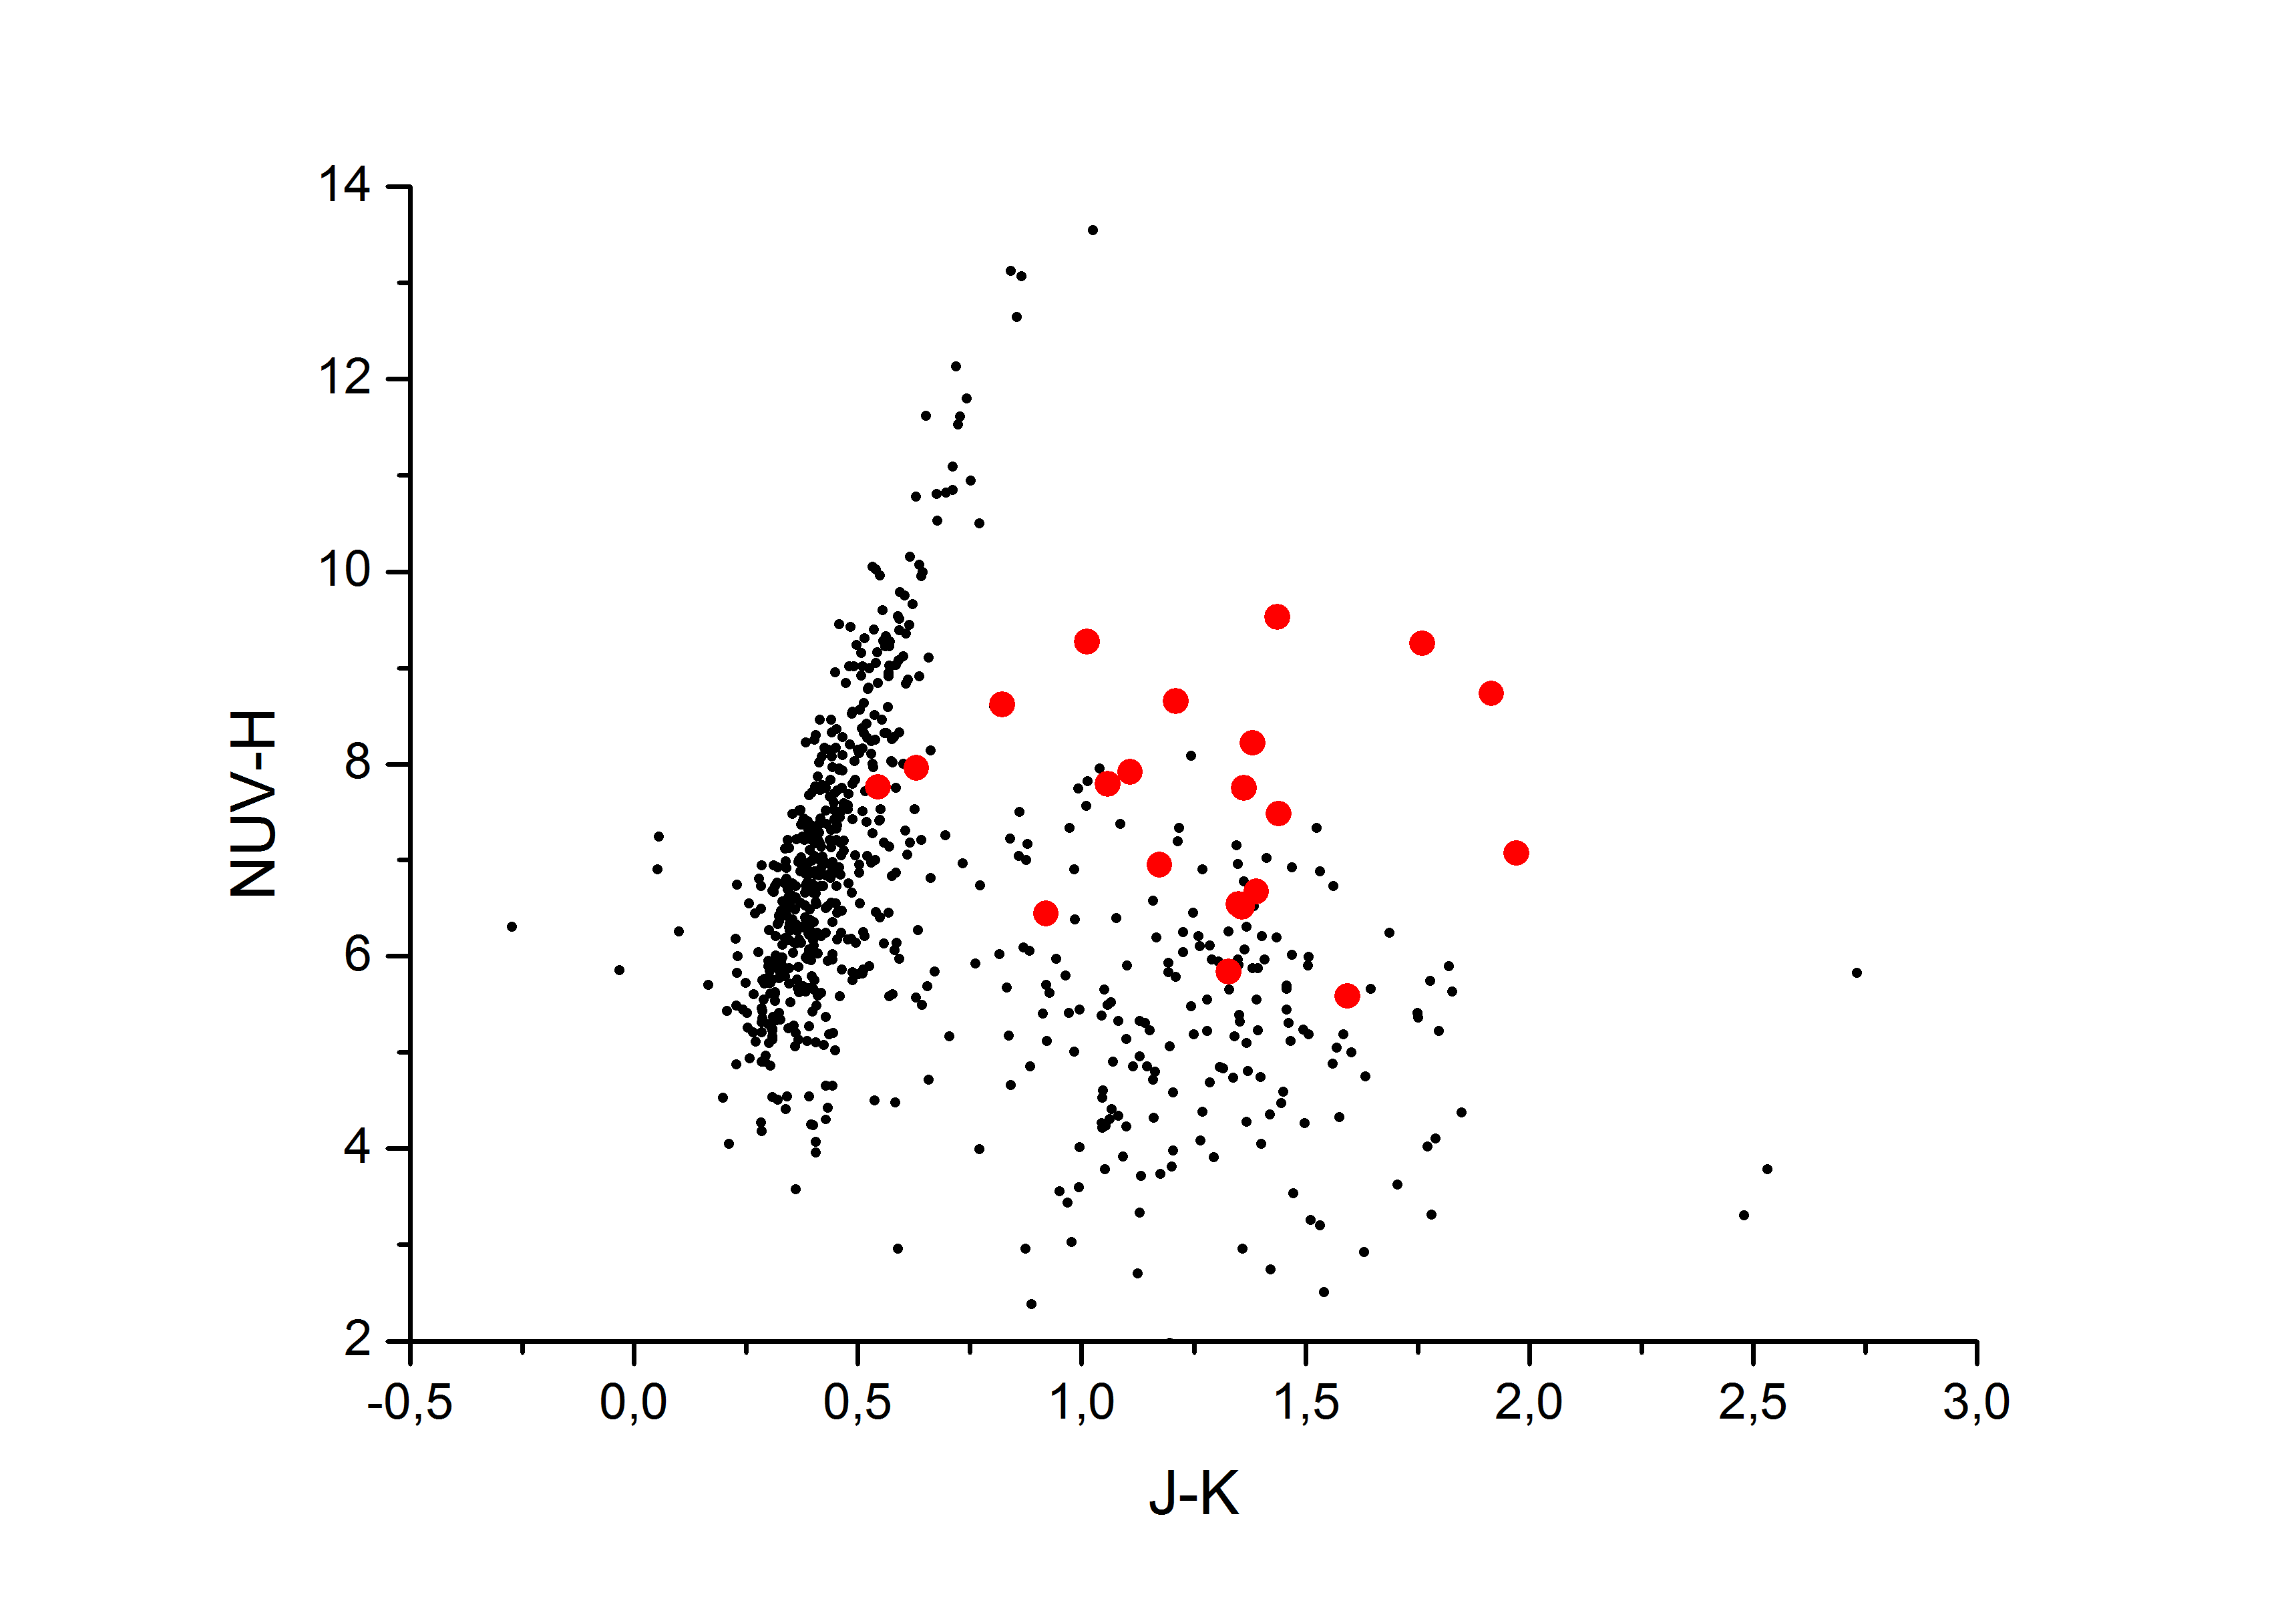
\includegraphics[width=1\linewidth]{Graph3.png} \\ NUV-R vs J-K}
\end{minipage}
\caption{Диаграммы цвет-цвет}
\label{fig:colcol}
\end{figure}

Звёзды эталонной выборки выделены красным. Заметно, что они группируются в стороне от основной массы звёзд, относящихся к главной последовательности. Также можно видеть, что довольно много звёзд находятся в той же области диаграммы, что и эталоны.

На диаграмме NUV-H vs J-K эталонные T Tauri особенно сильно отделены от остальных звёзд, поэтому критерий, относящийся к этой диаграмме, должен оказаться самым сильным.


Теперь мы можем сформулировать критерии первичного отбора кандидатов:
\begin{itemize}
	\item FUV-NUV vs J-K: звёзды типа Т Тельца должны удовлетворять 0.5 < J - K < 2.4 и 0.4 < FUV - NUV < 4.6;
	\item	FUV-NUV vs H-K: звёзды типа Т Тельца должны удовлетворять 0.2 < H - K < 1.2 и 0.4 < FUV - NUV < 4.6;
	\item	NUV-R vs J-K: звёзды типа Т Тельца должны удовлетворять 0.5 < J - K < 2.4 и 1.5 < NUV - R < 8.2;
	\item	NUV-H vs J-K: звёзды типа Т Тельца должны удовлетворять 0.5 < J - K < 2.4 и 4.2 < NUV - H < 11.0;
\end{itemize}

Наша цель -- не только найти кандидаты в T Tauri звёзды, мы хотим, чтобы ни одна из них не была потеряна в ходе отбора, если это возможно. Поэтому на этом этапе мы оставляем те источники, которые удовлетворяют хотя бы одному из четырёх критериев.

\section{Результат и адекватность критериев}
Получили столько-то источников. Самый сильный критерий оказался третий (вроде)

Не упускают ли критерии известные звёзды типа Т Тельца? В нашей области проверить не на чем, но вот люди (Ана Инес) проверили на TMC и работает.
